\section{Aktuelle Situation und Vergleich}
		\subsection{IOS}
			\subsubsection{Emulation}
			Die Emulation von iOS-Geräten ist derzeit mit der Verwendung von XCode möglich. XCode wiederum ist nur unter Mac OSX erhältlich. Da Max OSX laut EULA nur auf "Apple-branded computers" verwendet werden darf \cite{AppleEULA}, ist die Simulation von iOS-Geräten nur unter Apple-Hardware möglich. Nach der Installation über den in Mac OSX enthaltenen App-Store kann ein virtualisierter IPhone über die Schritte XCode, Open Developer Tools, Simulator gestartet werden.
		\subsubsection{Debugging}
Als Debugger unter Mac OS X hat sich LLDB etabliert und stellt das Pendant zu GDB unter Linux dar. LLDB ist kostenlos verfügbar, Open-Source und steht unter der https://opensource.org/licenses/UoI-NCSA.php Lizenz, welche die Vervielfältigung und Veränderung des Quellcodes unter unter Hinweis auf LLVM erlaubt.

LLDB sollte auf jedem Mac OS X System mit XCode automatisch installiert sein und lässt sich im Terminal über das Kommando
\begin{lstlisting}
lldb
\end{lstlisting} aufrufen. Eine Gegenüberstellung von GDB-Kommandos zu LLDB steht unter \url{http://lldb.llvm.org/lldb-gdb.html} zur Verfügung.
\\
 Kompiliert man eine Applikation in XCode, wird diese in einem emulierten IPhone gestartet und direkt ein Fenster LLDB hergestellt. Die ausgeführte Applikation ist in LLDB automatisch ausgewählt.

\begin{figure}[htbp]
	\centering
	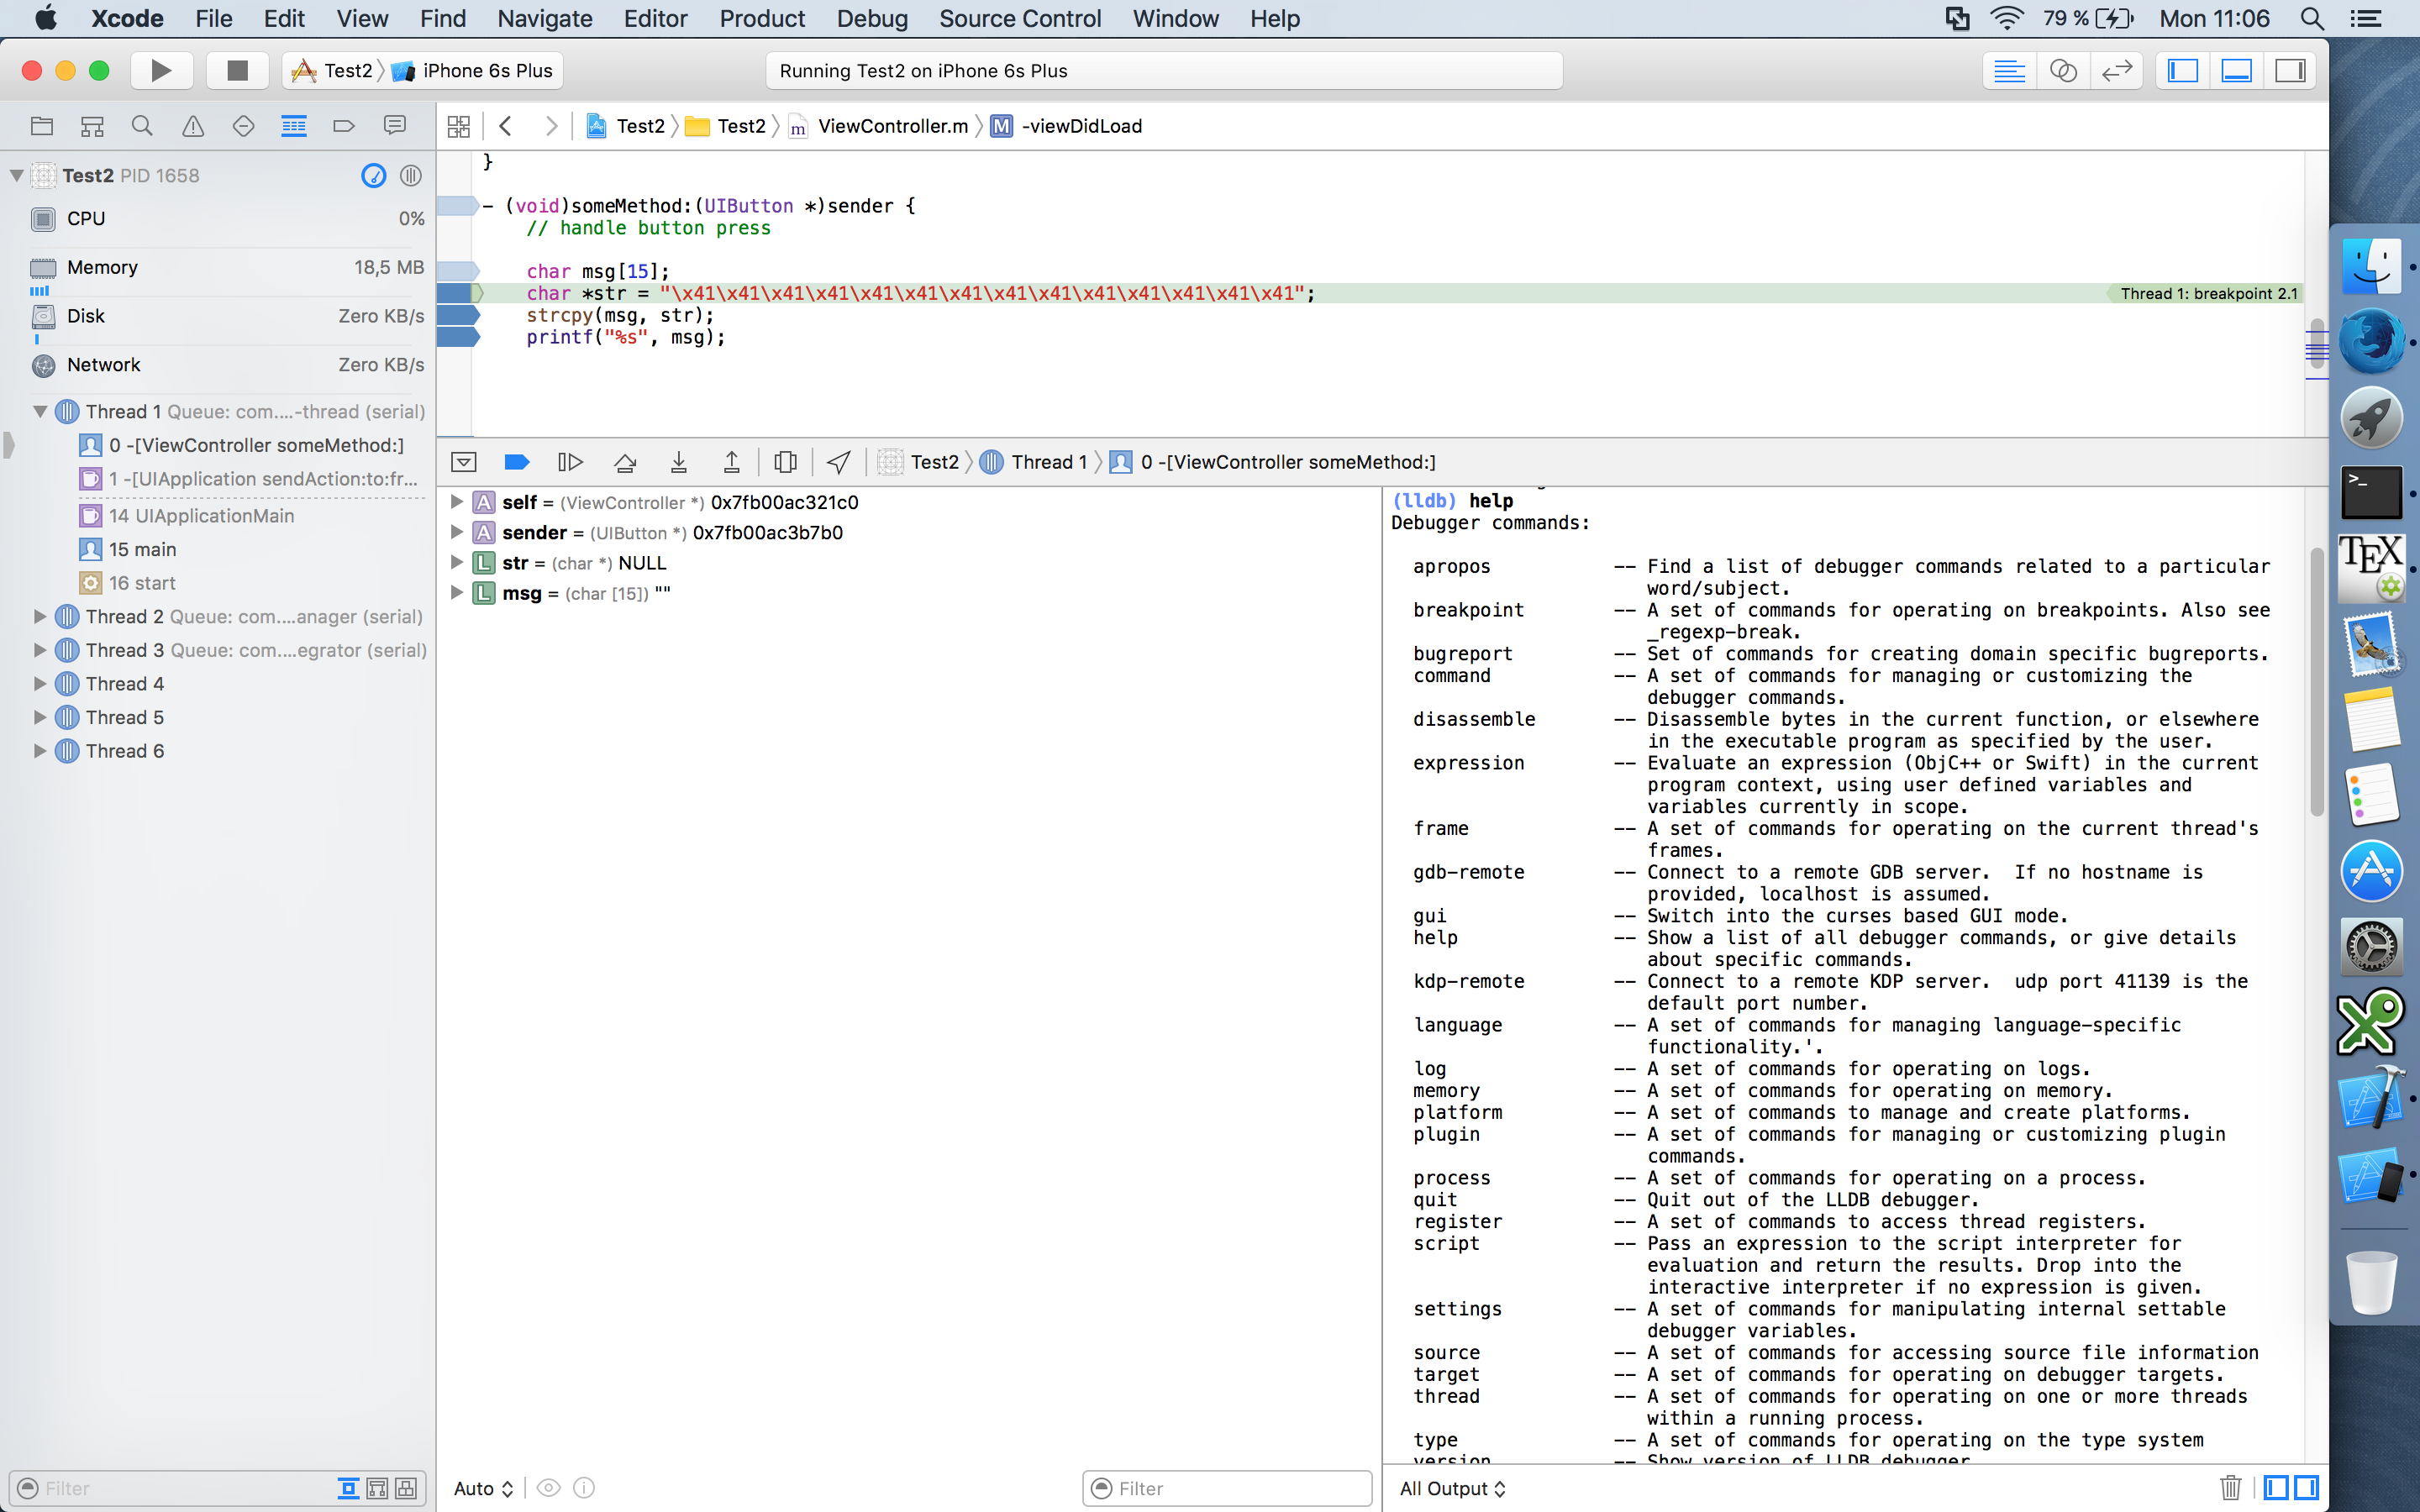
\includegraphics[width=\textwidth]{bilder/pentest_mobile_anwendungen/vergleich_aktuelle_situation/20160627_XCode-LLDB.png}
	\caption{LLDB in XCode}
	\label{fig:LLDBinXCode}
\end{figure}
Ein Ziel dieser Arbeit ist jedoch das Automatisieren von Analysen, weshalb das Ausführen der grafischen Oberfläche nicht optimal ist.

Leider ist nicht erkennbar, wie LLDB und das emulierte IPhone eine Verbindung herstellen. Eine Auflistung der offen Sockets auf dem System legt jedoch nahe, dass auf dem IPhone das Programm \textit{debugserver} gestartet wird, welches Remote-Debugging mit LLDB erlaubt. Es bleibt herauszufinden, wie die Debugging-Session auf dem simulierten IPhone ohne XCode hergestellt werden kann.

\begin{figure}[htbp]
	\centering
	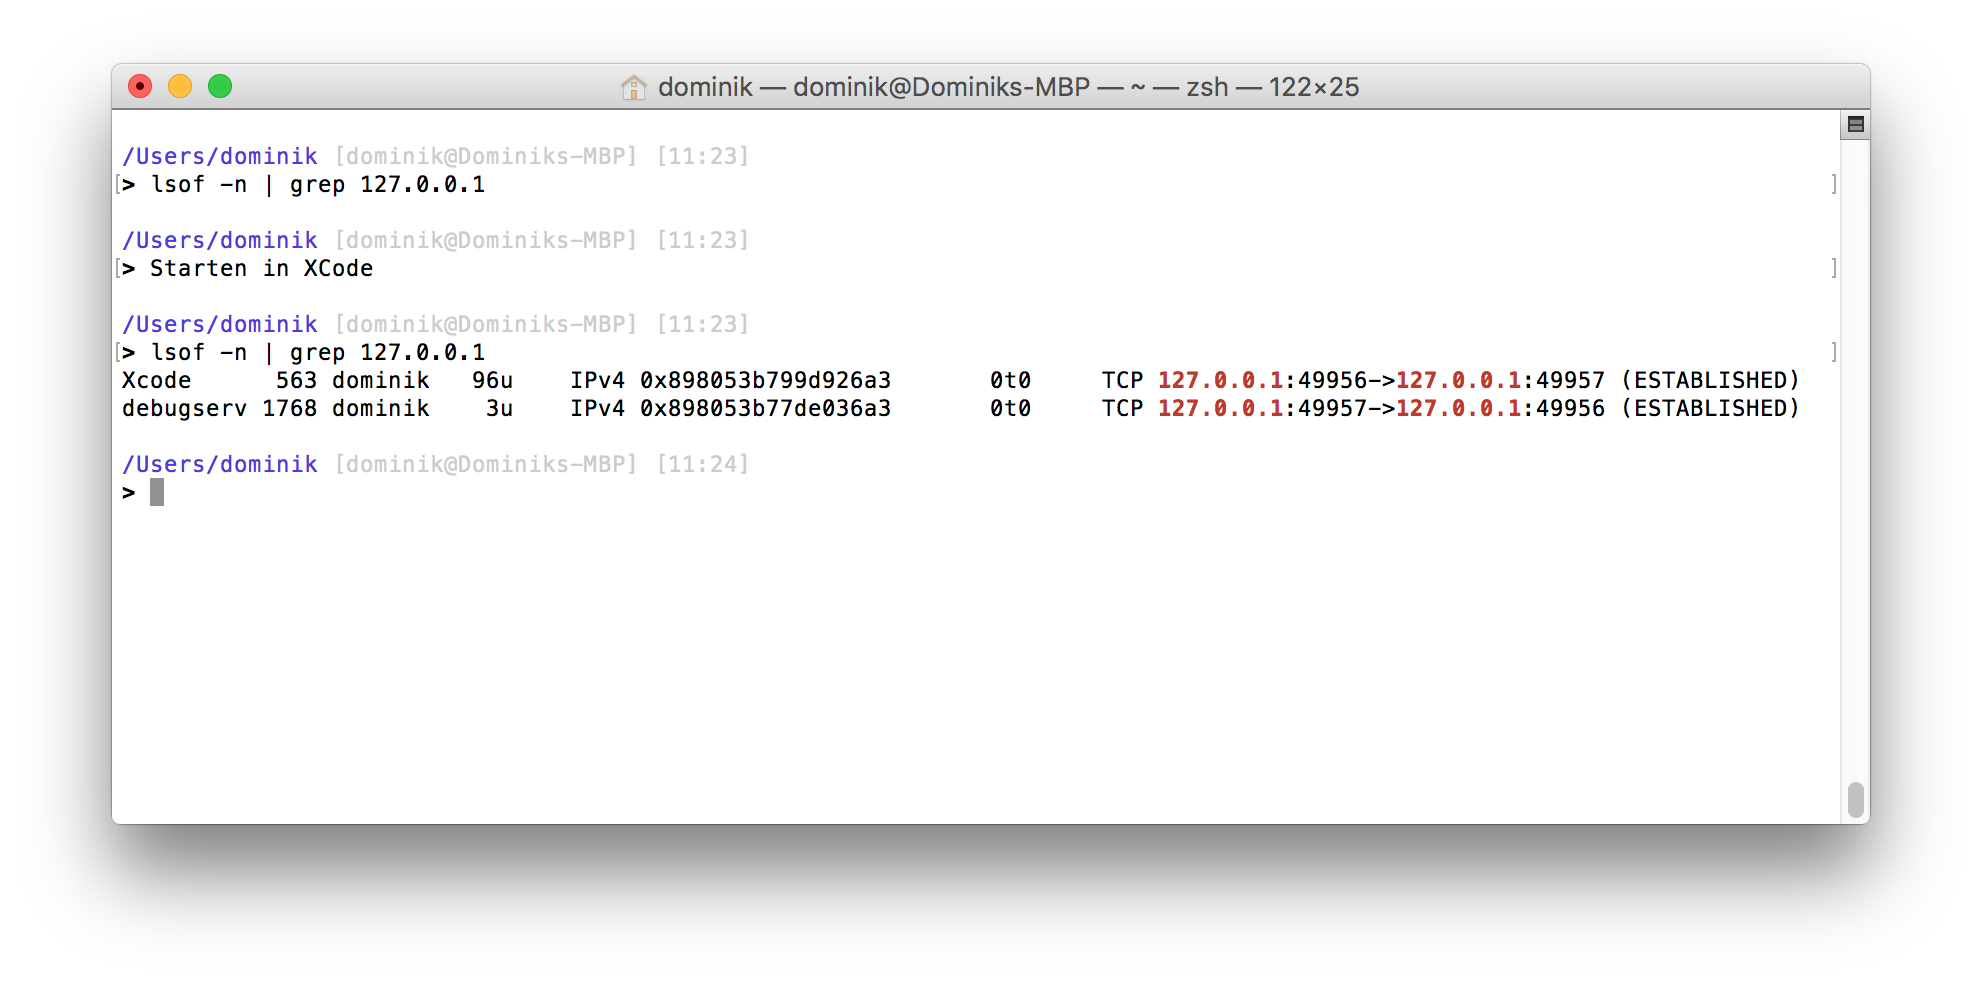
\includegraphics[width=\textwidth]{bilder/pentest_mobile_anwendungen/vergleich_aktuelle_situation/20160627_lsof_XCode_running.png}
	\caption{Vergleich der offenen Pipes vor und nach der Ausführung der Applikation in XCode}
	\label{fig:LSOFLLDB}
\end{figure}

Nach dem Artikel \url{https://developer.apple.com/library/ios/documentation/IDEs/Conceptual/gdb_to_lldb_transition_guide/document/lldb-terminal-workflow-tutorial.html} von Apple, ist es möglich, mit  LLDB eine App auch als "Standalone Debugger", also ohne XCode, zu verwenden. Dies ist in Abbildung \ref{fig:LLDBStandaloneDebugger} aufgezeigt.

\begin{figure}[htbp]
	\centering
	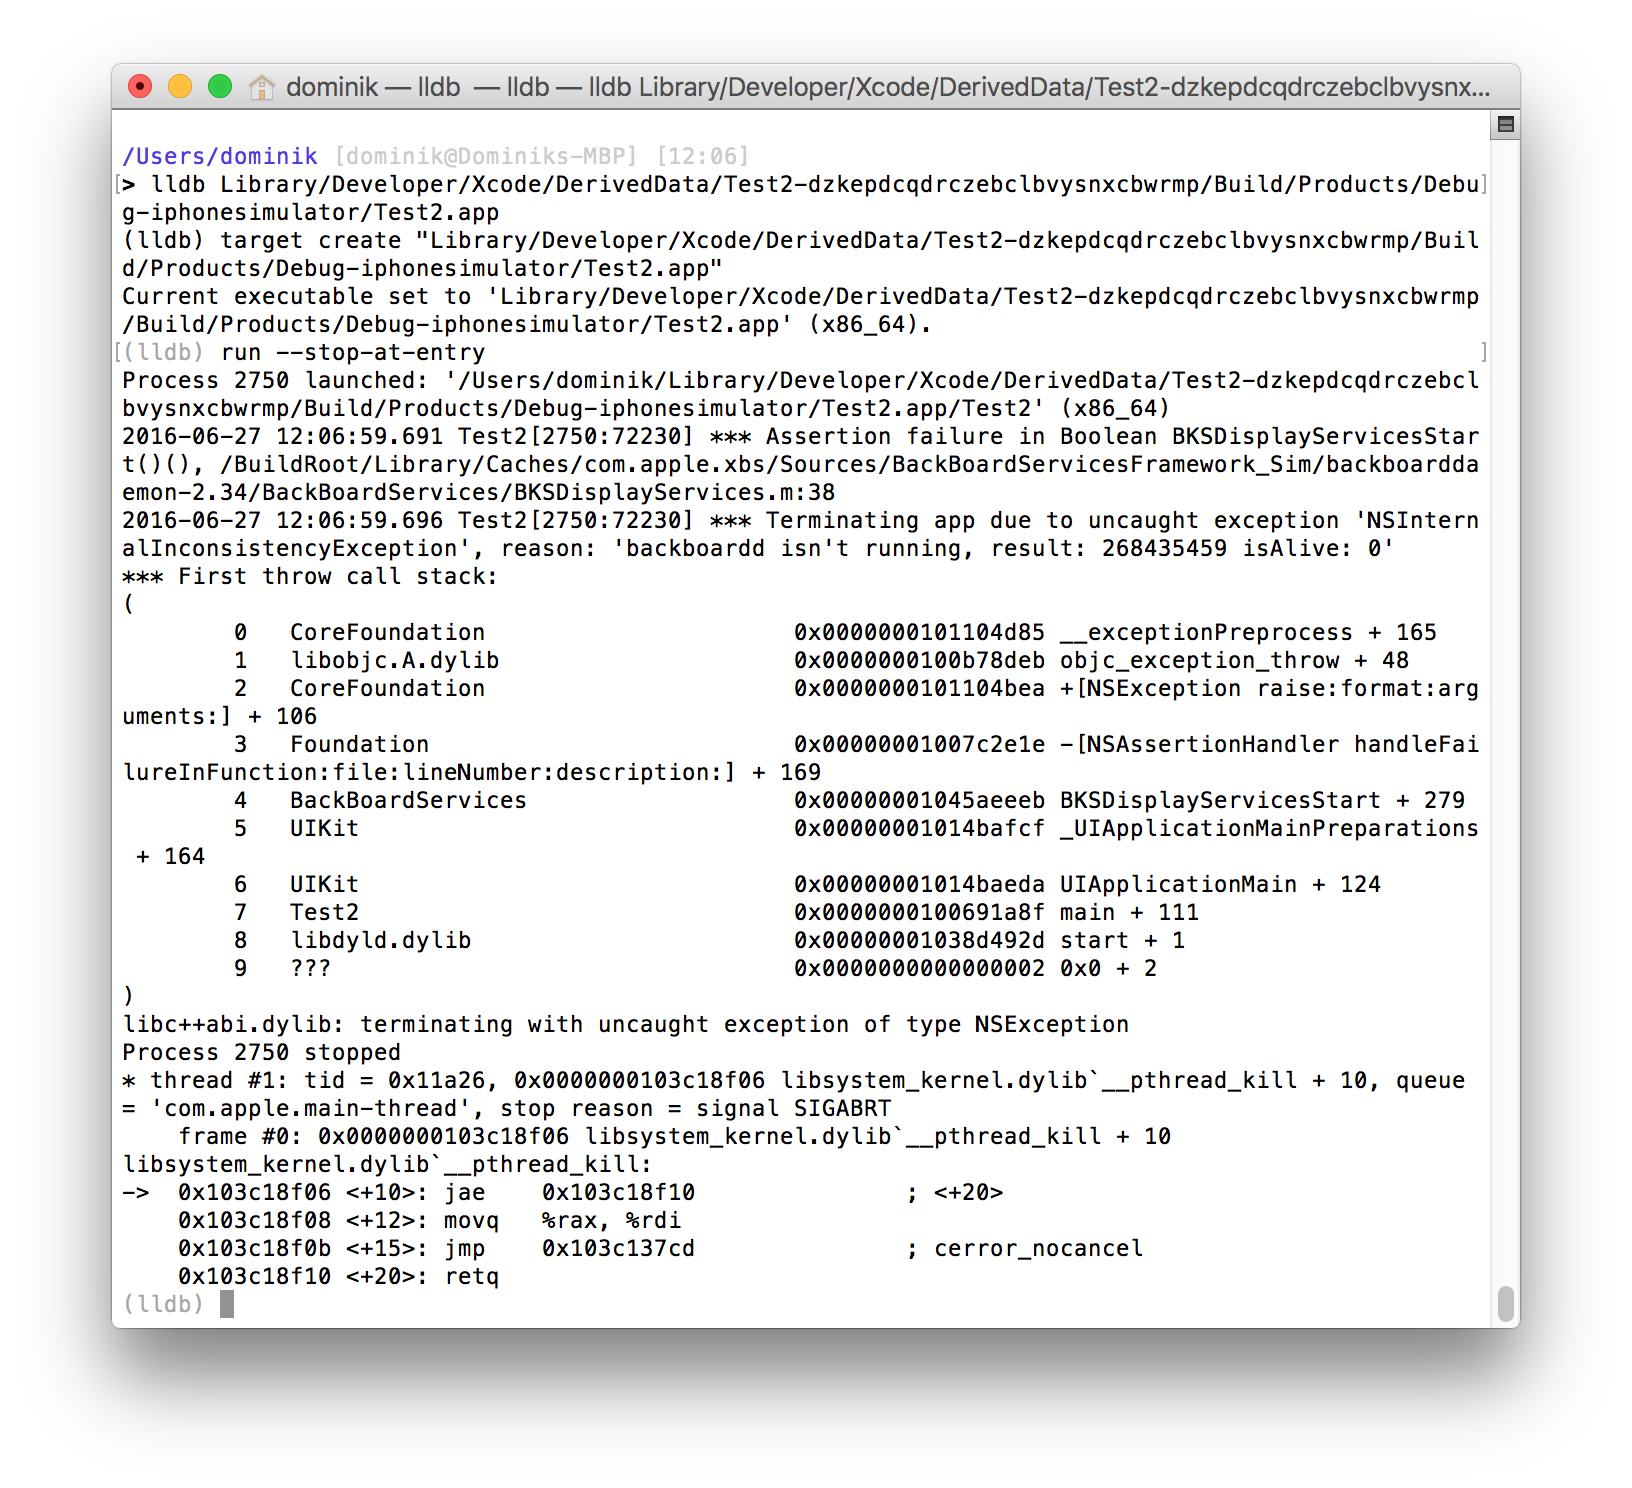
\includegraphics[width=\textwidth]{bilder/pentest_mobile_anwendungen/vergleich_aktuelle_situation/20160627_LLDB-Standalone-Debugger.png}
	\caption{LLDB als Standalone Debugger}
	\label{fig:LLDBStandaloneDebugger}
\end{figure}

Um zu verifizieren, dass die App auf einem simulierten IPhone ausgeführt wird, können entweder die geöffneten Prozesse (siehe Abbildung \ref{fig:LLDB-creating-IPhone-VM}) oder die geladenen Bibliotheken der Programme (siehe Abbildung \ref{fig:VergleichLLDBImages}) verglichen werden.

\begin{figure}[htbp]
	\centering
	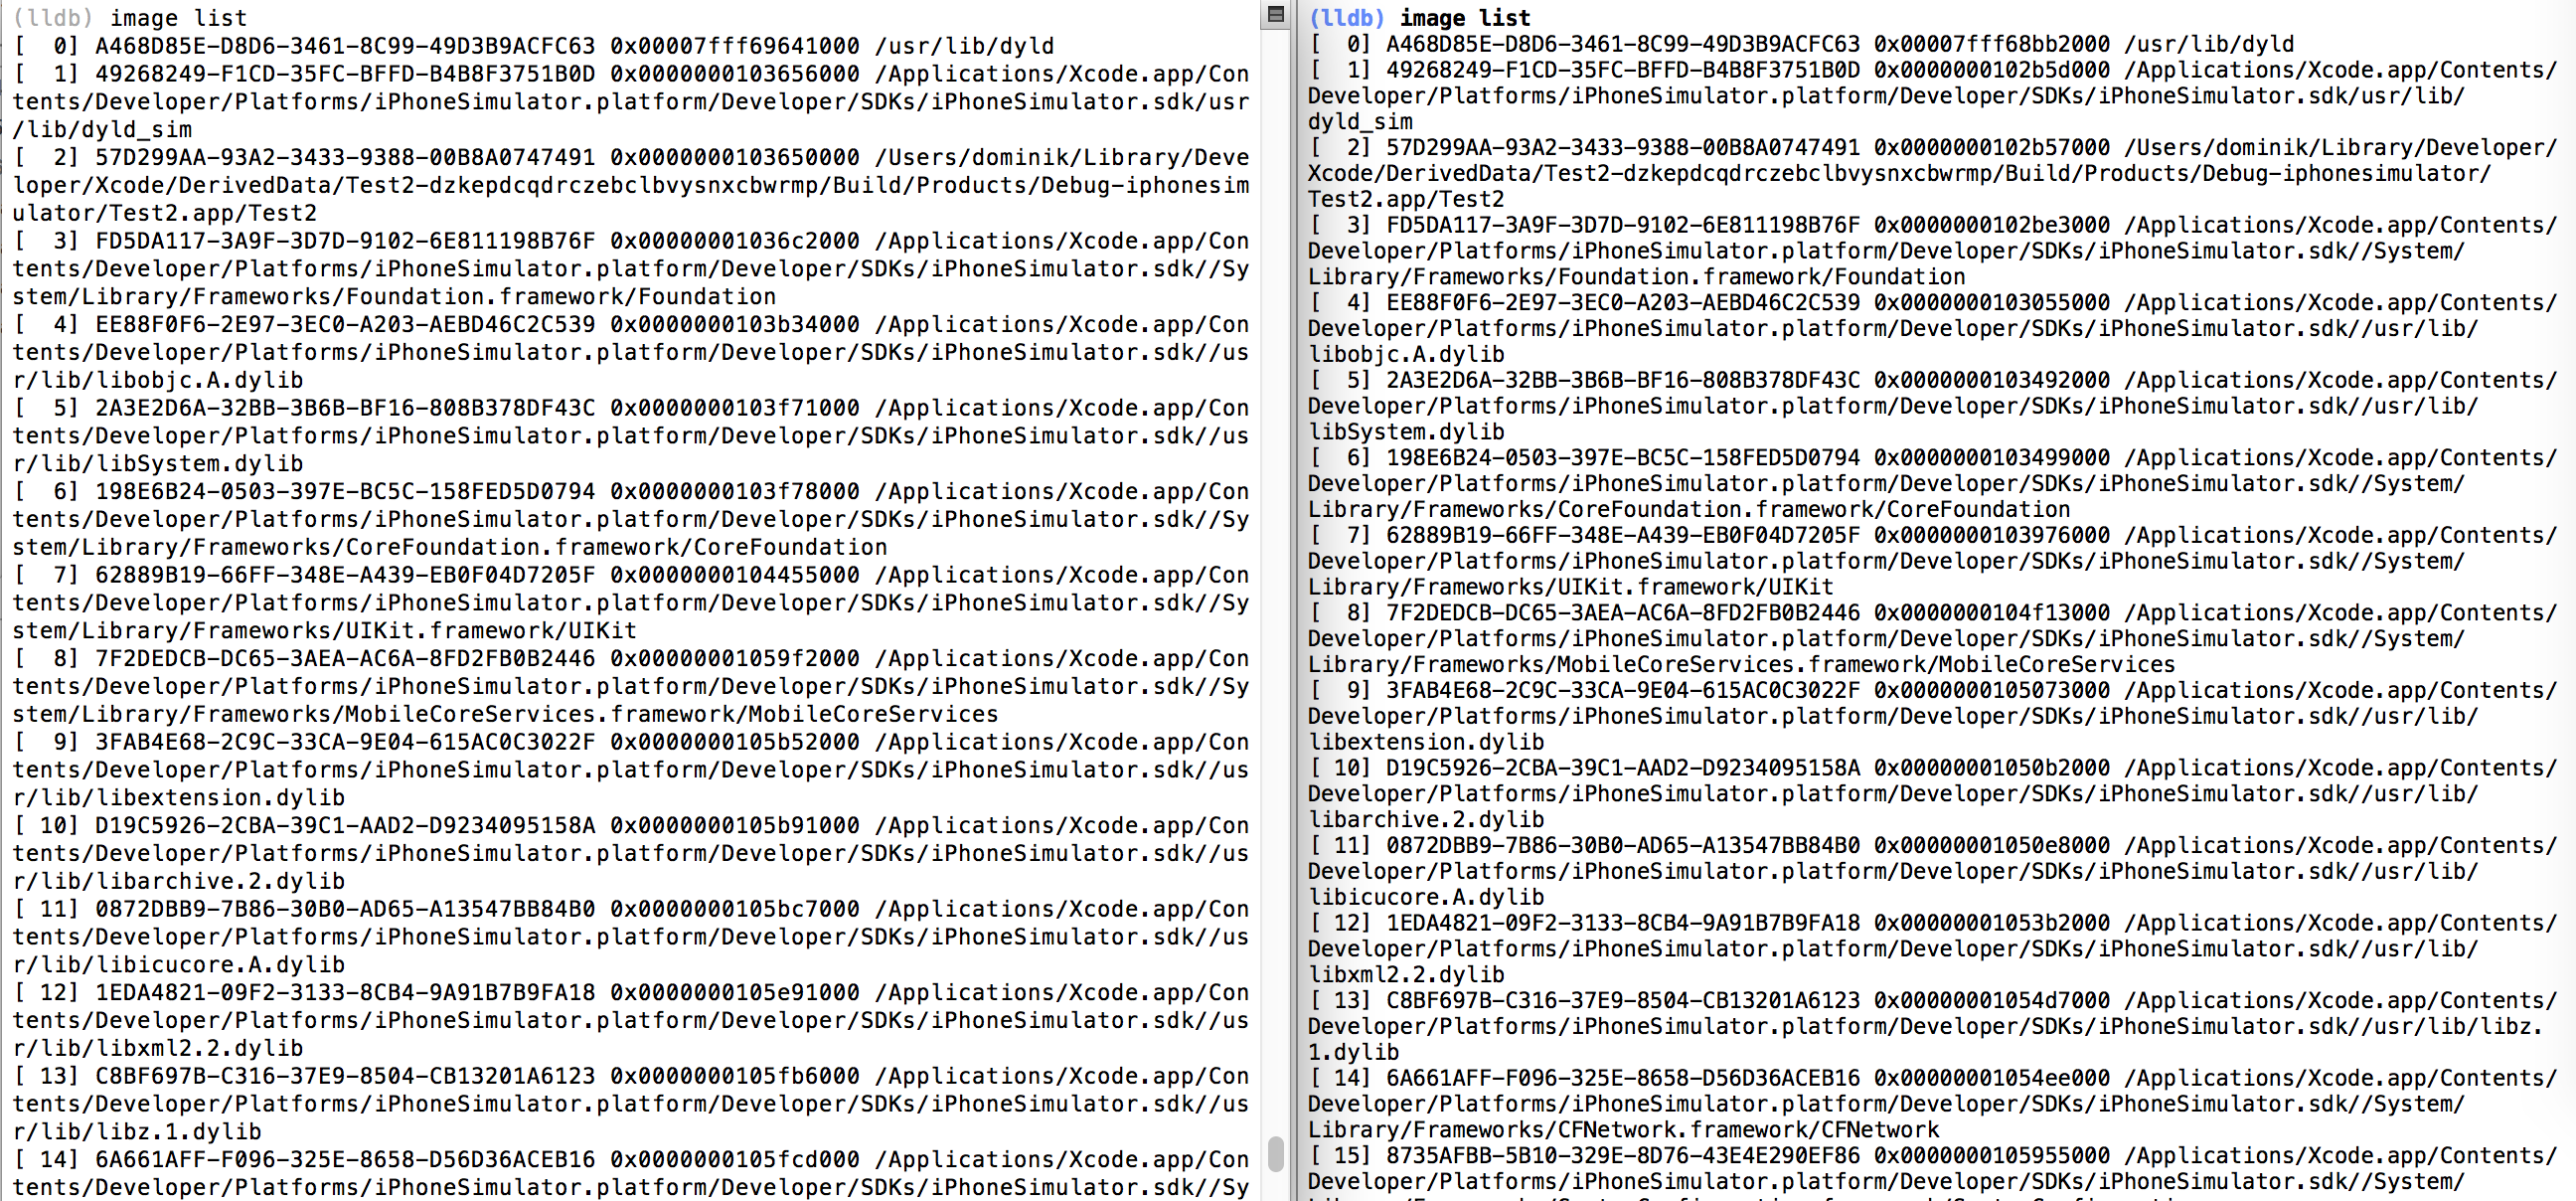
\includegraphics[width=\textwidth]{bilder/pentest_mobile_anwendungen/vergleich_aktuelle_situation/20160627_LLDB-image-list.png}
	\caption{LLDB als Standalone Debugger}
	\label{fig:VergleichLLDBImages}
\end{figure}

Bei Methoden zeigen, dass die App auf dem simulierten IPhone gestartet wird. Bei den Prozesse ist zu beobachten, dass vor Start von LLDB nur der Hintergrund-Service ausgeführt wurde. Nach dem Start von LLDB dagegen, läuft der gesamte Simulator.

Auch der Vergleich der geladenen Libaries legt nahe, dass die LLDB Standalone und XCode in der gleichen Umgebung ausgeführt werden. Die Adressen im RAM variieren aufgrund von ASLR zwar, aber es werden die Bibliotheken verwendet (am Pfad zu erkennen).

\begin{figure}[htbp]
\lstinputlisting[caption={Gestartete Prozesse nach LLDB Aufruf},lastline=16]{logs/20160627_LLDB-creating-IPhone-VM.txt}
\label{fig:LLDB-creating-IPhone-VM}
\end{figure}

\paragraph{Memory Corruption}
Bad Functions


\paragraph{Ungesicherte Verbindungen}$ $\\
https://developer.apple.com/library/ios/documentation/General/Reference/InfoPlistKeyReference/Articles/CocoaKeys.html unter NSAppTransportSecurity

\begin{lstlisting}
NSURL *url = [NSURL URLWithString:@"http://api.ipify.org"];
    NSData *data = [NSData dataWithContentsOfURL:url];
    NSString *ret = [[NSString alloc] initWithData:data encoding:NSUTF8StringEncoding];
    NSLog(@"ret=%@", ret);
\end{lstlisting}

\begin{lstlisting}
2016-06-28 08:42:56.518 Test2[4789:140270] App Transport Security has blocked a cleartext HTTP (http://) resource load since it is insecure. Temporary exceptions can be configured via your app's Info.plist file.
\end{lstlisting}


		\subsection{Windows-Phone}
			\subsubsection{Emulation vs. Hardware}
			VS
			\subsubsection{Debugging}
			VS	
		\subsection{Android}
			Android ist ein Ursprünglich 2003 von der Android, Inc. entwickeltes mobiles Betriebssystem. 2005 wurde es durch Google übernommen und wird seit dem weiterentwickelt. 2015 liegt es bei einem Marktanteil von TODO \%. Aufgrund der Quelloffenheit des Systems wird von vielen Herstellern auf verschiedensten Plattformen genutzt. Jedoch bringt die weitführende Fragmentierung des Betriebssystems auch Nachteile mit sich. So sind in 2015 nur TODO \% der Android-Devices auf einer aktuellen Version.\cite{Drake2014}
			\subsubsection{Android-Studio und SDK}
			Das Android-Studio ist eine umfassende IDE. Sie ermöglicht unter anderem das schnelle Entwickeln und Testen von Apps, sowie die Emulation von beliebigen Android-Versionen. Außerdem ist Android Studio kostenlos, Open-Source und für Linux, Mac und Windows erhältlich. Die aktuelle Version kann unter \url{http://developer.android.com/sdk/index.html} heruntergeladen werden. Die Installation unter Linux ist vergleichsweise einfach, da nur ein Archiv über das Kommando 
\begin{lstlisting}
unzip android-studio-ide-143.2739321-linux.zip
\end{lstlisting}
entpackt werden muss. Für alle anderen Betriebssysteme werden entsprechende Installationsroutinen zur Verfügung gestellt. Anschließend kann die IDE über die Datei "`bin/studio.sh"' gestartet werden. Neben dem Android-Studio gibt es noch das Android SDK, welches über die gleiche URL heruntergeladen werde kann. Es enthält wichtige Kommandozeilen-Tools wie \textit{adb}, \textit{fastboot} oder \textit{logcat}, auf welche im weiteren Verlauf noch detailliert eingegangen wird.
			\subsubsection{Compatibility Testing Suite}
			\cite{Drake2014} Seite 18
			\subsubsection{Emulation vs. Hardware}
			Android SDK
			\subsubsection{Debugging}	
			Android Debug Bridge\cite{androidDebugBridge}
			\subsubsection{Logcat}	
			Android Debug Bridge\cite{androidDebugBridge}